\section{Electrostatic potential}

\begin{framenologo}
  \frametitle{Electrostatic potential}
  \tableofcontents[currentsection]
\end{framenologo}

\subsection{Boundary conditions}

\begin{frame}
  \frametitle{Electrostatic potential}
  \framesubtitle{Boundary conditions}

  Boundary conditions are fulfilled via:
  \begin{itemize}[<+->]
    \item<.-> Electrodes behave bulk

    \item Extended electrode regions helps the above

    \item Corrections to the Hartree potential are necessary (TranSiesta solves Poisson
    equation via Fourier transforms, i.e. periodic)

    \item Always remember that the self-energy \emph{forces} the boundary conditions,
    i.e. a long range decay-potential may be forced too short

  \end{itemize}

  \uncover<.->{
  \begin{center}

    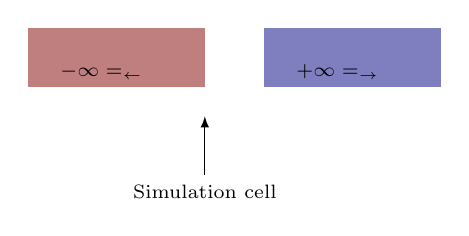
\begin{tikzpicture}[z=.5cm,>=latex,scale=.75,font=\scriptsize]
      \drawcube[draw]
      \begin{scope}[xshift=-3cm,x=3cm]
        \begin{scope}
          \drawcube[draw,densely dotted]
          \fill[red!50!black,fill opacity=0.5] (0,0,1) -- (1,0,1) -- (1,1,1) -- (0,1,1)
          -- cycle;
        \end{scope}
      \end{scope}
      \begin{scope}[xshift=1cm,x=3cm]
        \begin{scope}
          \drawcube[draw,densely dotted]
          \fill[blue!50!black,fill opacity=0.5] (0,0,1) -- (1,0,1) -- (1,1,1) -- (0,1,1)
          -- cycle;
        \end{scope}
      \end{scope}

      % Draw arrows
      \node[anchor=center] at (-1.5,.5,.5) {$-\infty=\SE_\leftarrow$};
      \node[anchor=center] at (2.5,.5,.5) {$+\infty=\SE_\rightarrow$};

      \draw[<-] (0.5,0,0.) -- ++(0,-1,0) node[below] {Simulation cell};
      % \draw[->] (.5,.5,.5) -- (1.5,.5,.5);
      % \draw[->] (.5,.5,.5) -- (.5,1.5,.5);

    \end{tikzpicture}

  \end{center}}

\end{frame}


\begin{frame}
  \frametitle{Electrostatic potential}
  \framesubtitle{Boundary conditions}

  \begin{block}<+->{Hartree potential}

    NEGF calculations are \emph{very} different from periodic calculations because of the
    semi-infinite leads.

  \end{block}

  \begin{block}<+->{Boundary conditions}

    The electrode Hartree potential are the boundary conditions.

    In TranSiesta this is accomplished by fixing the electrostatic potential at one of the
    electrode planes.

    \begin{itemize}
      \item For $N_\idxE=2$ and aligned semi-infinite directions the potential profile can
      easily be approximated by a linear ramp $V(x) = ax+b$.

      \item For un-aligned semi-infinite directions (or $N_\idxE\neq2$) the potential
      profile cannot easily be approximated.

      \begin{itemize}[<+->]
        \item By default, TranSiesta implements a \emph{box} solution (bad guess) which
        only defines the boundary conditions on the electrode atoms. I.e. sets the Hartree
        potential equal to the chemical potential in the cell region of the electrode.

        \item A much better approach is to provide an \emph{external} potential profile
        guess, i.e. solve the boundary conditions using external Poisson
        solvers\footnote{\uncover<4->{This may seem like a more daunting task than it
                is. The guess is the Poisson solution \emph{without} charges, only the
                boundary conditions.}}

        \item \sisl\ has a tool to ease this. \shell{stoolbox ts-fft} may be used to
        create a better boundary condition as direct input for TranSiesta.

      \end{itemize}
    \end{itemize}
    
  \end{block}
  
\end{frame}


\subsection{Multi-electrode electrostatic potential}

\begin{frame}
  \frametitle{Electrostatic potential}
  \framesubtitle{Multi-electrode electrostatic potential}

  \begin{itemize}
    \item 6-electrode system
    \item Default \emph{box} solution for the Poisson equation
    \item External Poisson solution with electrode regions correct chemical potential
  \end{itemize}

  \begin{center}
    \incg[width=.8\linewidth]{ts-poisson-initial}
  \end{center}

  \begin{block}<2->{Help needed!}

    This is where TranSiesta could benefit the most from external help!

    A proper, Poisson solver with arbitrary boundary conditions.
    
  \end{block}
  
\end{frame}

